\documentclass[tikz,border=2pt]{standalone}
\usepackage{pgfplots}
\pgfplotsset{compat=1.18}
\usetikzlibrary{intersections}
\usepgfplotslibrary{fillbetween}

\begin{document}
	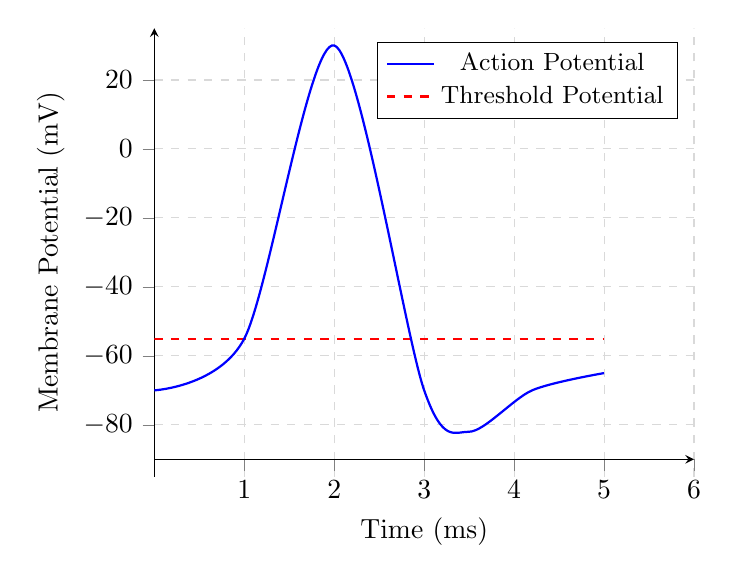
\begin{tikzpicture}
		\begin{axis}[
			axis lines=middle,
			ymin = -95,
			ymax = 35,
			xmin = 0,
			xmax= 6,
			grid = major,
			grid style={dashed, gray!30},
			ylabel near ticks,
			xlabel near ticks,
			xlabel= Time (ms),
			ylabel= Membrane Potential (mV),
			tick align=outside,
        			axis x line shift=90,
			legend pos= north east,
			legend style={font=\small, cells={align=left}},]

			\draw [red, thick, dashed](0,-55) -- (5,-55);
			\draw[blue, thick] plot[smooth,tension=0.5] coordinates { (axis cs: 0,-70) (axis cs: 1,-55) (axis cs: 2,30) (axis cs: 3,-70) (axis cs: 3.5,-82) (axis cs: 4.2,-70) (axis cs: 5,-65)};

		\addlegendimage{blue, thick};
		\addlegendentry{Action Potential};
		\addlegendimage{red, dashed, thick};
		\addlegendentry{Threshold Potential};


		\end{axis}
	\end{tikzpicture} 
\end{document}